\documentclass{article}
\usepackage{amsmath, cancel, graphicx, mathtools}
\usepackage{amssymb}

\graphicspath{{./imgs}}
\begin{document}
\section{10.a}
\[
    \frac{x^2 + x - 6}{x - 2} = x + 3
\]
\text{This equation is false if } x = 2 \\
\chaper{Singularity may happened in type }
\[
    \frac{c}{0} \quad ; \; c \in \mathbb{R}
\]


\section{10.b}
\[
    \lim_{x \to 2} \frac{x^2 + x - 6}{x - 2}
    =
    \lim_{x \to 2} x + 3
\]
\\
\text{Is corrected because when x is approcing to 2 means it's not equals 2
    so it's not make any singularity
} \\

\begin{align}

    \lim_{x \to 2} \dfrac { (x + 3) \cancel{(x - 2)} } { \cancel{(x - 2)} }
    =
    \lim_{x \to 2} (x + 3) \\

    \lim_{x \to 2} (x+3) = \lim_{x \to 2} x + 3 \\

    5 = 5 \\

\end{align}

\section{36.a}
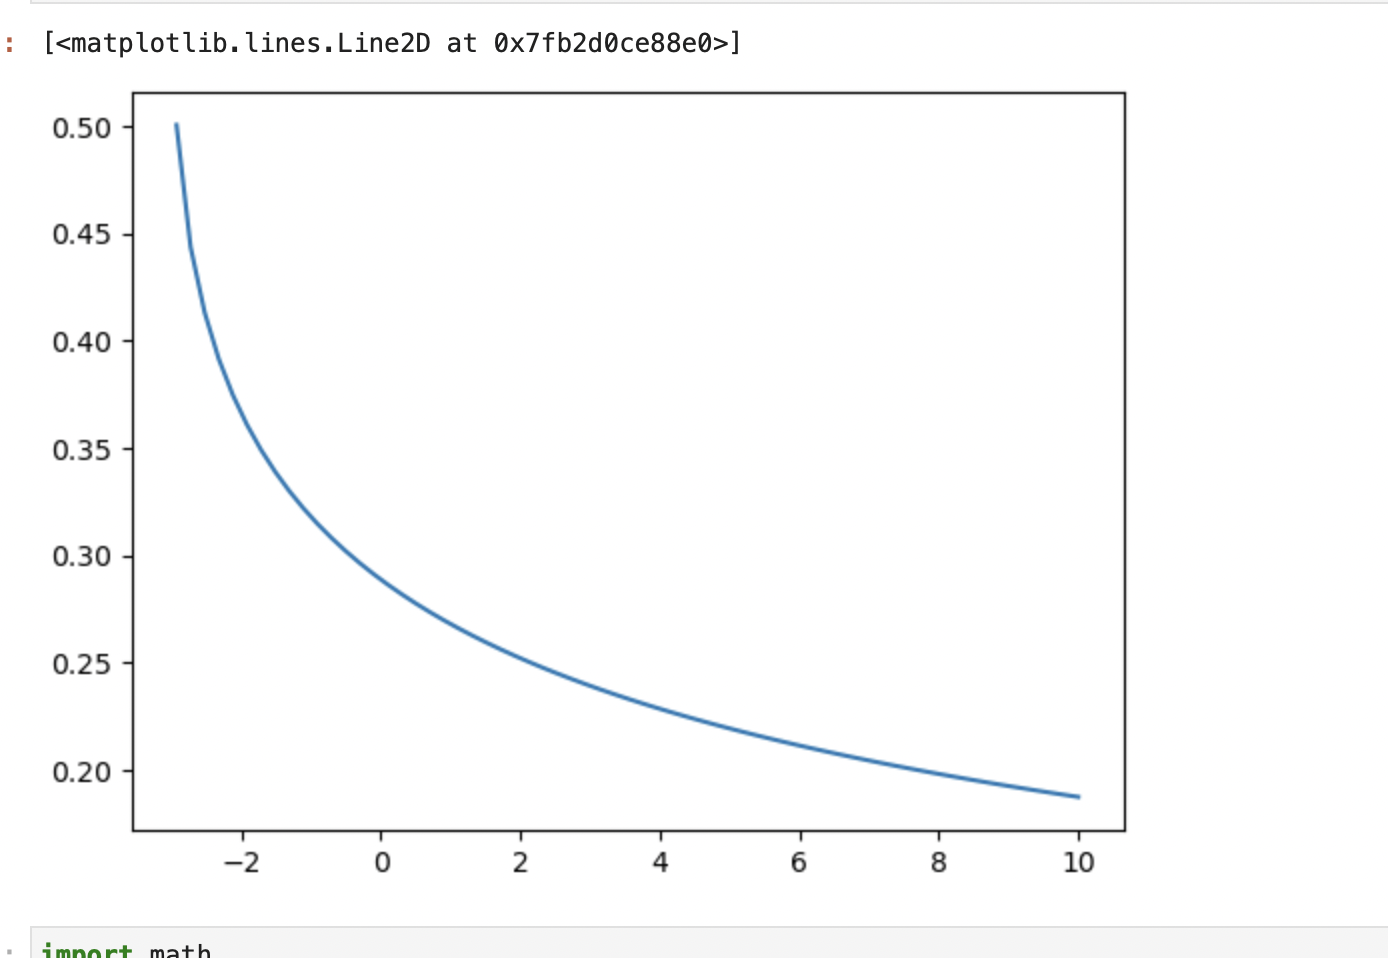
\includegraphics[scale=0.3]{graph.png}
\[
    \lim_{x \to 0} f(x) = 0
\]

\section{36.b}
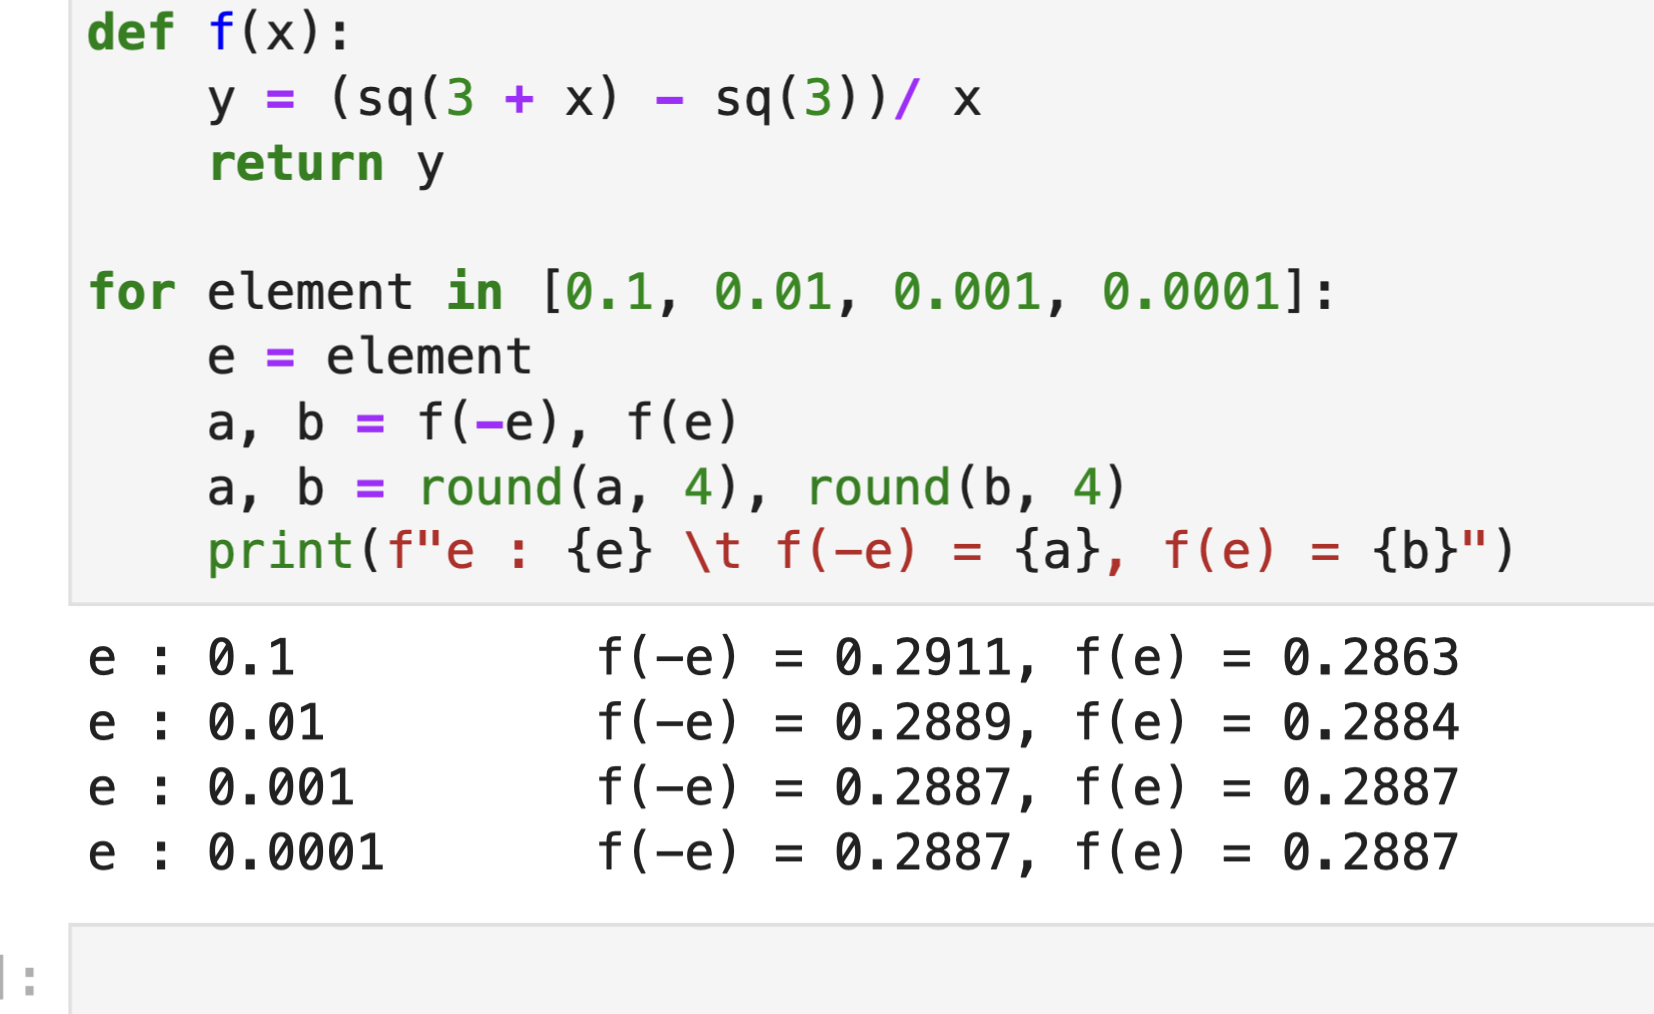
\includegraphics[scale=0.3]{table.png} \\
\text{from table we can see the pattern that if e is approch to 0 \\
then limit value is almost the same at 0.2887
}

\section{36.c}
\text{consider} f(x) \\

\begin{equation}
    \label{eq1}
    \begin{split}
    f(x) &= \dfrac{ \sqrt{3 + x} - \sqrt{3} }{ x } \\

    &= \dfrac {
        (\sqrt{3 + x} - \sqrt{3})
        (\sqrt{3 + x} + \sqrt{3})
    }
    {
        (x)
        (\sqrt{3 + x} + \sqrt{3})
    } \\


    &= \dfrac{
        (3 + x) - 3
    }
    {
        (x)
        (\sqrt{3 + x} + \sqrt{3})
    } \\

    &= \dfrac{
        x
    }
    {
        (x)
        (\sqrt{3 + x} + \sqrt{3})
    } \\

    &= \dfrac{ 1 }
    {
        (\sqrt{3 + x} + \sqrt{3})
    }
    \end{split}
\end{equation}

\begin{equation}
    \label{eq2}
    \begin{split}
    \lim_{x \to 0} f(x) &= \dfrac{ 1 } { (\sqrt{3 + 0} + \sqrt{3}) } \\
    &= \dfrac{ 1 } { (\sqrt{3} + \sqrt{3}) } \\
    &= \dfrac{ 1 } { 2\sqrt{3} } \\
    &\approx 0.2887
    \end{split}
\end{equation}
\end{document}
